\documentclass{beamer}
\mode<presentation>
\usepackage{amsmath}
\usepackage{amssymb}
%\usepackage{advdate}
\usepackage{graphicx}
\usepackage{adjustbox}
\usepackage{subcaption}
\usepackage{enumitem}
\usepackage{multicol}
\usepackage{mathtools}
\usepackage{listings}
\usepackage{url}
\def\UrlBreaks{\do\/\do-}
\usetheme{Boadilla}
\usecolortheme{lily}
\let\vec\mathbf
\setbeamertemplate{footline}
{
  \leavevmode%
  \hbox{%
  \begin{beamercolorbox}[wd=\paperwidth,ht=2.25ex,dp=1ex,right]{author in head/foot}%
    \insertframenumber{} / \inserttotalframenumber\hspace*{2ex} 
  \end{beamercolorbox}}%
  \vskip0pt%
}
\setbeamertemplate{navigation symbols}{}

\providecommand{\nCr}[2]{\,^{#1}C_{#2}} % nCr
\providecommand{\nPr}[2]{\,^{#1}P_{#2}} % nPr
\providecommand{\mbf}{\mathbf}
\providecommand{\pr}[1]{\ensuremath{\Pr\left(#1\right)}}
\providecommand{\qfunc}[1]{\ensuremath{Q\left(#1\right)}}
\providecommand{\sbrak}[1]{\ensuremath{{}\left[#1\right]}}
\providecommand{\lsbrak}[1]{\ensuremath{{}\left[#1\right.}}
\providecommand{\rsbrak}[1]{\ensuremath{{}\left.#1\right]}}
\providecommand{\brak}[1]{\ensuremath{\left(#1\right)}}
\providecommand{\lbrak}[1]{\ensuremath{\left(#1\right.}}
\providecommand{\rbrak}[1]{\ensuremath{\left.#1\right)}}
\providecommand{\cbrak}[1]{\ensuremath{\left\{#1\right\}}}
\providecommand{\lcbrak}[1]{\ensuremath{\left\{#1\right.}}
\providecommand{\rcbrak}[1]{\ensuremath{\left.#1\right\}}}
\theoremstyle{remark}
\newtheorem{rem}{Remark}
\newcommand{\sgn}{\mathop{\mathrm{sgn}}}
\providecommand{\abs}[1]{\vert#1\vert}
\providecommand{\res}[1]{\Res\displaylimits_{#1}} 
\providecommand{\norm}[1]{\lVert#1\rVert}
\providecommand{\mtx}[1]{\mathbf{#1}}
\providecommand{\mean}[1]{E[ #1 ]}
\providecommand{\fourier}{\overset{\mathcal{F}}{ \rightleftharpoons}}
%\providecommand{\hilbert}{\overset{\mathcal{H}}{ \rightleftharpoons}}
\providecommand{\system}[1]{\overset{\mathcal{#1}}{ \longleftrightarrow}}
%\providecommand{\system}{\overset{\mathcal{H}}{ \longleftrightarrow}}
	%\newcommand{\solution}[2]{\vec{Solution:}{#1}}
%\newcommand{\solution}{\noindent \vec{Solution: }}
\providecommand{\dec}[2]{\ensuremath{\overset{#1}{\underset{#2}{\gtrless}}}}
\newcommand{\myvec}[1]{\ensuremath{\begin{pmatrix}#1\end{pmatrix}}}


\lstset{
%language=C,
frame=single, 
breaklines=true,
columns=fullflexible
}
\lstset{
  language=C,
  basicstyle=\ttfamily\footnotesize,
  keywordstyle=\color{blue}\bfseries,
  commentstyle=\color{gray}\itshape,
  stringstyle=\color{orange},
  numbers=left,
  numberstyle=\tiny\color{gray},
  breaklines=true,
  frame=single,
  showstringspaces=false,
  tabsize=4,
  captionpos=b
}
\numberwithin{equation}{section}
\lstset{
  language=Python,
  basicstyle=\ttfamily\small,
  keywordstyle=\color{blue},
  stringstyle=\color{orange},
  numbers=left,
  numberstyle=\tiny\color{gray},
  breaklines=true,
  showstringspaces=false
}

\title{Problem 2.7.7}
\author{Sujal Rajani}

\date{\today} 
\begin{document}

\begin{frame}
\titlepage
\end{frame}


\section{Question}
\begin{frame}{Question}
\textbf{Question}:
\\

\noindent Find the area of the quadrilateral ABCD whose vertices are $\vec A$(-4,-3), $\vec B(3,-1)$,$\vec C$(0,5), and $\vec D$(-4,2).
\end{frame}
\section{Solution}
\begin{frame}{Solution}
\textbf{Solution:} 

as given in the question :
\begin{align*}
     \vec{A}=\myvec{-4\\-3\\0},
     \vec{B}=\myvec{3\\-1\\0},
     \vec{C}=\myvec{0\\5\\0},
     \vec{D}=\myvec{-4\\-2\\0}
\end{align*}
the position vector joining $\vec{B}$ and $\vec{D}$ =  $\vec{B}$ -  $\vec{D}$ =$\myvec{7\\1\\0}$ 
\\
\\
\\
the position vector joining $\vec{C}$ and $\vec{A}$ =  $\vec{C}$ -  $\vec{A}$ =$\myvec{4\\8\\0}$
\\
\\
\\
\\
the area of quadrilateral ABCD is the vector  product of $\dfrac{1}{2}$($\vec{B}$ -  $\vec{D}$)X($\vec{C}$ -  $\vec{A}$)
\\  
\end{frame}
\begin{frame}{Solution}
\subsection{VECTOR PRODUCT }
\textbf{VECTOR PRODUCT}
\\
let N be a vector :
\begin{align}
    \vec{N}=\myvec{n_1\\n_2\\0}
    \\
    \end{align}
    let M be a vector :
    \begin{align}
    \vec{M}=\myvec{m_1\\m_2\\0}
\end{align}
the vector product of two vectors $\vec{N}$ and $\vec{M}$ is 
\\
\vec{N}X\vec{M} =
\myvec{
n_{23} & m_{23} \\
n_{31} & m_{31} \\
n_{12} & m_{12}
}
=
\myvec{
n_2 m_3 - n_3 m_2 \\
n_3 m_1 - n_1 m_3 \\
n_1 m_2 - n_2 m_1
}
=
\myvec{
1 \times 0 - 0 \times 8 \\
0 \times 7 - 7 \times 0 \\
7 \times 8 - 1 \times 4
}
=
\myvec{
0 \\
0 \\
52
}
\end{frame}
\begin{frame}{Solution}
{area of ABCD is :}
\begin{align*}
     \dfrac{1}{2}||(\vec{B}-  \vec{A})X(\vec{C} -  \vec{A})||=\dfrac{1}{2}||\myvec{7\\1\\0}X\myvec{4\\8\\0}||= \dfrac{1}{2}\sqrt{\myvec{0\\0\\52}^T\myvec{0\\0\\52}}=26
    \end{align*}
    \\
    n1=7,n2=1,m1=4,m2=8

\end{frame}
    \subsection{plot}
       \begin{frame}[fragile]
    \begin{figure}[H]
    \centering
    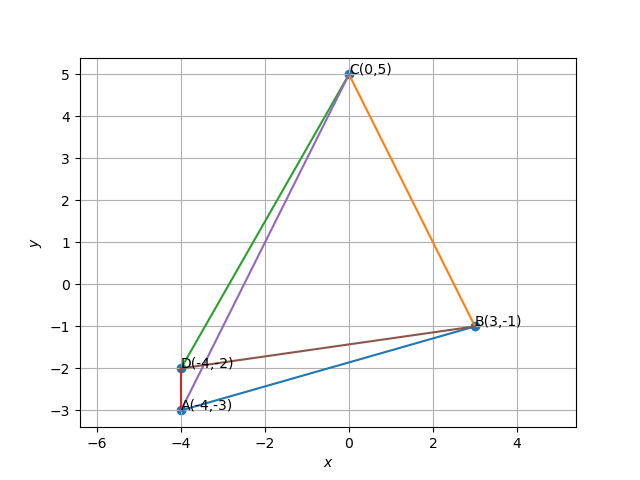
\includegraphics[width = 0.6\columnwidth]{../figs/img.png}
    \caption*{}
    \label{figs}
\end{figure}
\end{frame}
\section{ C Code}
\begin{frame}[fragile]
\frametitle{C Code }
\begin{lstlisting}[language=C]
#include <stdio.h>
#include <stdlib.h>

int main() {
    // Vertices
    int Ax = -4, Ay = -3;
    int Bx = 3, By = -1;
    int Cx = 0, Cy = 5;
    int Dx = -4, Dy = 2;

    // Diagonals as vectors: AC and BD
    int ACx = Cx - Ax; // 0 - (-4) = 4
    int ACy = Cy - Ay; // 5 - (-3) = 8
    int BDx = Dx - Bx; // -4 - 3 = -7
    int BDy = Dy - By; // 2 - (-1) = 3

    
\end{lstlisting}
\end{frame}

\begin{frame}[fragile]
\frametitle{C Code }
\begin{lstlisting}[language=C]
    
// Cross product of AC and BD (scalar value)
    int cross = ACx * BDy - ACy * BDx;

    // Area is half the magnitude of the cross product
    double area = 0.5 * abs(cross);

    printf("Area of the quadrilateral by scalar product = %.2lf square units\n", area);

    return 0;
}
    
\end{lstlisting}
\end{frame}



\begin{frame}[fragile]
\frametitle{Python Code for Plotting}
\begin{lstlisting}[language=Python]
import math
import sys   

import numpy as np
import numpy.linalg as LA
import matplotlib.pyplot as plt
import matplotlib.image as mpimg
from line.funcs import *
#from triangle.funcs import *
#from conics.funcs import circ_gen
#if using termux
import subprocess
import shlex
#end if

A = np.array([-4,-3]).reshape(-1,1)
B = np.array([3,-1]).reshape(-1,1)


\end{lstlisting}

\end{frame}
\section{Python Code}
\begin{frame}[fragile]
\frametitle{Python Code for Plotting}
\begin{lstlisting}[language=Python]
C = np.array([0,5]).reshape(-1,1)
D = np.array([-4,-2]).reshape(-1,1)
coords = np.block([[A,B,C,D]])


AB = line_gen(A,B)
BC = line_gen(B,C)
CD = line_gen(C,D)
DA = line_gen(D,A)
AC = line_gen(A,C)
BD = line_gen(B,D)

plt.plot(AB[0,:],AB[1,:])
plt.plot(BC[0,:],BC[1,:])
plt.plot(CD[0,:],CD[1,:])

\end{lstlisting}

\end{frame}
\begin{frame}[fragile]
\frametitle{Python Code for Plotting}
\begin{lstlisting}[language=Python]
plt.plot(DA[0,:],DA[1,:])
plt.plot(AC[0,:],AC[1,:])
plt.plot(BD[0,:],BD[1,:])

plt.scatter(coords[0,:],coords[1,:])


plt.text(A[0],A[1],"A(-4,-3)")
plt.text(B[0],B[1],"B(3,-1)")
plt.text(C[0],C[1],"C(0,5)")
plt.text(D[0],D[1],"D(-4,-2)")

plt.xlabel('$x$')
plt.ylabel('$y$')
plt.legend(loc='best')
plt.grid() # minor
plt.axis('equal')

plt.savefig('../figs/img.png')


\end{lstlisting}

\end{frame}
\begin{frame}[fragile]
\frametitle{Python Code for Plotting}
\begin{lstlisting}[language=Python]
plt.legend(loc='best')
plt.grid() # minor
plt.axis('equal')

plt.savefig('../figs/img.png')

\end{lstlisting}

\end{frame}
\end{document}